% !TEX root = ../../my-thesis.tex

\graphicspath{{./content/conclusion/fig/}}

\chapter{Discussion}
\label{sec:conclusion}

\cleanchapterquote{To be but one with all living things, to return, by a radiant self-forgetfulness, to the All of Nature.}{Friedrich Hölderlin (1770-1843)}{}


\section{Contributions}
Understanding biological and economic systems involves the underpinning of the elemental processes underlying the systems' macroscopic features, and establishing the associated mechanisms (\cite{Levin2002}, \cref{fig:forward_inverse_modelling}).
% 
Following this approach, my work aimed at advancing our understanding of how ecological and evolutionary processes, and their interplay, shape the dynamics of biological and economic systems. In particular, this thesis contributed to 
% 
\begin{mylisti}
    \item a fundamental undersanding of the role of eco-evolutionary processes in shaping the dynamics of biological populations structured in complex landscapes \cref{chap:diff-in-graphs},
    \item the quantification of the effect of mechanisms associted with eco-evolutionary processes in economic systems \cref{chap:econobiology},
    \item methodological advances in the forward and inverse modelling of eco-evolutionary dynamics \cref{chap:diff-in-graphs,chap:mini-batching,chap:nonlocalPDE}.
\end{mylisti}

In the following, I discuss the chapters of my thesis collectively within the broader context of our current understanding of the dynamics of biological and economic systems, and the accompanying modelling paradigm.

\subsection{Advancing our fundamental understanding of eco-evolutionary processes in biological and eocnomic systems}

\subsubsection{Linking eco-evolutionary processes to patterns of differentiation}
Spatial patterns of biodiversity result from the processes of selection, mutation and dispersal, that act upon individual organisms \citep{hamilton2021population}.
% \cref{\chapi} contributed to advance our understanding on how eco-evolutionary processes and population structure influence population dynamics and phenotypic evolution in biological systems.
% 
In finite size populations, mutations result in "drift" \citep{Slatkin1987a}, causing stochastic variations in the allelic proportions and phenotypes of biological populations. In geographically structured population, drift results in patterns of neutral differentiation \citep{Slatkin1987a}, where isolated populations are characterised by differentiated allelic proportions and phenotypes. 
% 
Dispersal tends to reduce neutral differentiation \citep{Slatkin1987a}, and this effect is modulated by landscape connectivity \citep{Wright1943,McRae2006,McRae2007} through the mechanism of "isolation by limited dispersal" \citep{Orsini2013}. By increasing the dispersal ability of organisms, landscape connectivity decreases neutral differentiation \citep{Lande1991}.
% 
When landscapes present heterogeneous habitats, natural selection can supplement the effect of genetic drift and increase the sole effect of stochasticity on differentiation \citep{fisher1958genetical}. Under this scenario, local environment conditions select individuals with traits that provide them higher fitness \citep{Gaither2018}. At the population level, this results in populations adapting to their local environment, a mechanism coined "local adaptation" \citep{Kawecki2004} and resulting in patterns of "adaptive differentiation". 
% 
% This results in adaptive differentiation, and is regarded as one of the most important factors govening species richness gradients \citep{Kawecki2004}.
% 
Adaptive differentiation is hindered by dispersal, which prevents local adaptation by bringing maladapted individuals, that destabilise the evolution of traits towards the optimal \citep{Meszena1997,Debarre2013,Mirrahimi2020}.
% 
% confounded by genetic drift, opposed by natural selection due to tempoeral envionrmental variability, and constrained by loack of genetic variation of by the genetic architecture of underlying traits \citep{Kawecki2004}. TODO: this may go in the perspective and limitations
% 
% Specifically, ref. \citep{Mirrahimi2020} presents a condition for local adaptation, where populations can locally adapt if the dispersal intensity $m$ is below a certain threshold involving the strength of natural selection $s$ and the strnegth of habitat heterogeneity $\theta$,
% \begin{equation}\label{eq:mirr_disp}
%     m < 2s\theta^2.
% \end{equation}
% 
While adaptive differentiation concerns traits under selection, it undirectly affects the differentiation of neutral traits, that are co-evolving with traits under selection through linkages \citep{Billiard2015,Lepers2021}. This results in turn to the mechanism of "isolation by adaptation", where habitat heterogeneity, rather than landscape connectivity, increases neutral differentiation \citep{nosil2008}. 
% 
Simple mechanisms resulting in neutral and adaptive differentiation are identified, but how they are modulated by eco-evolutionary feedbacks and landscape complexity is unclear. %TODO: unclear

In \cref{\chapi}, I demonstrate a novel mechanism, involving the process of intra-specific competition, that considerably affects neutral differentiation. Through the creation of unbalanced migration fluxes which increases the intensity of competition in highly connected populations, heterogeneity in connectivity reduces gene flow and reinforces neutral differentiation. %Through the accumulation of incompatibilities over time \citep{Dobhsanski}, this mechanism could lead to speciation over time, and contribute to the high diversification in mountain regions \citep{Rahbek}.
% 
I also investigate how the mechanism of local adaptation in complex landscapes, where habitats are arranged in a realistic fashion. I show that the complexity of habitat spatial distribution can be reduced to a measure of habitat spatial auto-correlation, coined the "habitat assortativity". Landscapes characterised by a high habitat assortativity systematically support populations that are locally better adapted than in landscape with low assortativity, resulting in higher adaptive differentiation. Specifically, I provide an analytical condition for local adaptation that sheds light on how it relates to dispersal intensity, selection strength, habitat heterogneity, and habitat assortativity.

Because habitat assortativity affects local adaptation, is must also affect neutral differentiation throuh the mechanism of isolation by adapation. Closing the loop, I demonstrate that habitat assortativity affects population differentiation through two antagonistic effects. By favoring local adaptation, it promotes isolation by adaptation, therefore increasing neutral differentiation. In parallel, it also favors gene flow within clusters of similar environmental conditions, decreasing isolation by limited dispersal. This results in habitat assortativity decreasing neutral differentiation for low dispersal intensity, and increasing neutral differentiation for high dispersal intensity.
% 
This complex feedback is essential to understand population differentiation in complex landscapes.

I provide a summary of the processes and resulting mechanisms shaping neutral and adaptive differentiation in \cref{fig:summary_diff-in-graph}. Overall, \cref{\chapi} links processes to patterns, establishing an extensive map of causal pathways involved in the phenotypic differentiation of populations. % It extends on recent work including the interplay between ecological and evolutionary processes, and frequency dependence, hihglighting non-trivial emergent properties with large consequences on emergent patterns.

\begin{figure}[t]
    \centering
    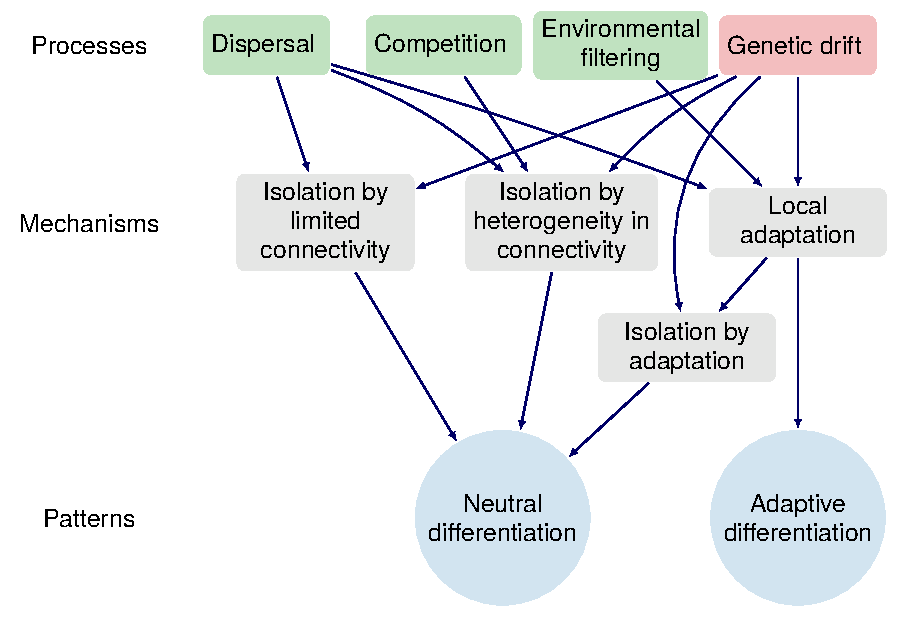
\includegraphics[width=\textwidth]{diff-in-graph.pdf}
    \caption{\textbf{Summary of the causal pathways involved in neutral and adaptive differentation, disentangled in \cref{\chapi}}. Ecological processes are displayed in green boxes, evolutionary processes are displayed in red boxes.}
    \label{fig:summary_diff-in-graph}
\end{figure}


\subsubsection{Linking economic patterns to eco-evolutionary processes}

% Hypotheses concerning the processes that underly economic system dynamics are numerous, and have mainly been investigated through forward modelling. Starting from empirical observations, 
% 
\cref{\chapiii} provides a novel understanding of the role of eco-evolutionary processes in economic systems. %by assessing their effect on the dynamics of economic activities from data.
% 
% complements recent follows an inverse modelling approach to understand which processes are most likely shaping economic development. 
% 
Neoclassical economics and evolutionary economics seek to explain economic change with formal modelling, focusing on the relationships between economic variables such as output, employment and productivity \citep{Boschma2005a}.
% 
% Neoclassical economics sugggests that exogenous drivers, such as production costs, drive the diversification of economic systems \xxx. 
% 
In particular, evolutionary economics is concerned with explaining economic change by endogenous forces, such as interactions between firms and economic activities, and evolutionary processes acting upon them \citep{Hodgson2019,Metcalfe2006}.
% 
% Exogenous drivers, such as technological change \xxx, economic institutions \xxx, and production costs \citep{Boschma2005a} have been proposed, but 
% 
In opposition to this approach, complexity economics \citep{Hidalgo2021} seeks to predict variations in national income by using fine-grained data of economic activity outputs and dimensionality reduction techniques \citep{Mitchell}, without making assumptions on the underlying processes \citep{Hidalgo}. 
% 
% One of the major contribution of complexity economics is to provide a metric that can predict economic development \citep{Taschella}, and the field is now concerned with understanding the factors underlying this factor.
%
While a current concern in evolutionary economics is to obtain an agreement between the mechanisms proposed and empirical observations \xxx, complexity economics seeks to understand the causal processes underlying the success of the dimensionality reduction technique \xxx.

By being agnostic to economic variables yet providing a causal link with the most probable processes underlying economic development, \cref{\chapiii} bridges evolutionary economics and economic complexity.
% 
Our approach relies on the simple observation that the dynamics of economic activities contains signatures from the many complex processes that underpin them.
% 
These signatures consist in peculiar temporal variations and couplings that can be conveniently modelled by biologically inspired population dynamic models, which use are additionally justified by deep analogies between economic activities and biological populations. 
% 
Analogously to biological populations that are characterised by genes, economic activities are characterised by organizational routines \citep{NelsonWinter}, which experience evolutionary processes and define how they engage in ecological processes \citep{NelsonWinter}.
% 
% This connection is justified by evolutionary economics, which argues that similarly to genes, organizational routines are at the core of economic entities and experience ecological and evolutionary processes.
% 
As a result, and similarly to the size of biological populations, the capital growth of economic activites is determined by the ensemble of organizational routines that characterise them \citep{Boschma2005a}.
% 
Similarly to approaches used in ecology and evolution \citep{Skeels}, inverse modelling approaches can then be used to disentangle, from their signatures \citep{Skeels} left on the dynamics of economic activities, the role of the eco-evolutionary processes acting upon them.

%%
Specifically, \cref{\chapiii} explores the effect of eco-evolutionary processes, proposed in the evolutionary economics and geography economics literature, on the dynamics of economic activities at the national scale.
% 
In particular, \cref{\chapiii} seeks to test whether the dynamics of economic activities can be explained by different types of interdependencies, including positive \xxx and negative interactions \xxx, spatial transfers \xxx, and economic transformations \xxx.
% 
Using population dynamic models capturing the different interdependencies, \cref{\chapiii} provides empirical evidence that economic activities engage in positive interactions, and benefit from spatial transfers of knowledge and routines.
% 
Positive interactions may arise from a variety of processes proposed in the evolutionary economic literature, such as supply chains \citep{Ozman2009,Saavedra2009a} and knowledge spillovers \citep{Menon2015}. 
% 
Its support implies that diversity promotes economic development \citep{Hidalgo2018}, as economic activities promote each other.
% 
The support for spatial transfers implies that, besides international patent laws \xxx, transfers of knowledge and organisational routines have a considerable effect on economic activities. Nevertheless, discrepancies in the strength-of-evidence obtained for spatial transfers across countries highlight that some countries are overall more akin to spatial transfers than others, which may be explained by differences in cognitive, organizational, social, institutional or geographic proximities across countries \xxx .
% 
I provide a summary of the mechanisms evidenced in economic systems in \cref{fig:summary_eco}. Overall, \cref{\chapiii} bridges approaches in economics and biology to understand the mechanisms shaping the endogenous dynamics of economic systems.

% 
% The dynamics of economic activities contains signals from the many complex processes that underpin them, this approach enables to extract the effect of economic processes through their 

% for the diffusion of countries through the product space, explaining technological lock out.
% 
% by using data and dimensionality reduction technique to leverage these assumptions \citep{Taschella},

\subsection{Leveraging forward and inverse modelling with ML}

\subsubsection{Advances in the modelling of realistic spatial and phenotypic structures}

\Cref{\chapi,\chapiv} provide new tools to better understand mechanisms resulting from ecological and evolutionary processes, and their interplay, in the context of realistic population structures and phenotypic distributions.
% 
% Population structure
Evolutionary dynamics have been traditionally studied in the context of regular population structures \citep{LiebermanHauert2005}.
% 
For instance, \cite{Slatkin1973,Slatkin1978,Kirkpatrick1997,Polechova2015,Polechova2018,AndradeRestrepo2019,Doebeli2003,Meszena1997,Yeaman2011,Debarre2013,Mirrahimi2020} consider regular spatial structures to investigate differentiation in biological populations, missing the effect of spatial complexity on the underlying mechanisms.
% 
Biological habitats differ in their connectivity \xxx, and economic entities are structured through complex networks \xxx. \cite{LiebermanHauert2005} and subsequent studies of "evolutionary dynamics on graphs" \xxx show that this complexity affects the interplay between selection and drift. However, evolutionary dynamics on graphs does not consider eco-evolutionary feedbacks \citep{Govaert2019a}.
% 
Thus far, models that include frequency dependence together with realistic, complex population structures were missing.

While a vast majory of the work on eco-evolutionary feedbacks has focused on the evolution of scalar phenotypes \citep{Doebeli2011}, in most organisms, many phenotypic properties combine in complicated ways to determine ecological processes \citep{Doebeli2014}.
% 
For instance, \cite{Doebeli2011} shows that the consideration of multiple traits is likely to generate more diversity than expected with one dimensional models.
% 
% \Cref{\chapi} also demonstrates that the co-evolution of traits proved to have genuine consequences on differentiation, pointing towards the inclusion of multiple traits to understand the dynamics of ecological interactions.
% 
Trade-offs in traits is also an essential feature shaping the evolutionary dynamics of biological populations, with consquences on the dynamics of e.g. cancer cell evolution \xxx and plankton dymamics \xxx.
% 
While there is overall a genuine need to better understanding evolutionary dynamics in high dimensional spaces, the simulation of high dimensional models is tremendously difficult, since the numerical cost of traditional methods grows exponentially in the number of dimensions of the phenotpic space. 
% 
% Novel numerical methods have been proposed to simulate high dimensional models, but they could not handle non-local terms, which capture non-local interactions between microscopic agents.

\cref{\chapi} develops a generic modelling framework to capture the effect of eco-evolutionary processes on biological populations structured in complex landscapes, and \cref{\chapiv} provides tools to efficiently simulate the resulting high-dimensional models.
% 
% TODO: this part does not work really well
%% IBM
The IBM presented in \cref{\chapi} involves the combination of graphs and highly dimensional phenotypic spaces, together with eco-evolutionary feedbacks, to model population structures. The modelling framework presented can readily be generalised, and the code associated to the numerical experiments in \cref{\chapi} include a Julia library, \textbf{Evoid.jl}, that implements a more general version of the model. %(), 
% 
As such, the modelling framework presented in \cref{\chapi} may be used to investigate other questions involving complex population structures and the co-evolution of characterisitcs.
% 
%% PDE
Reproducing the discrete and stochastic nature of ecological and evolutionary processes \citep{Champagnat2006}, simulations of the IBM may not provide a general understanding of system investigated \xxx, and cannot be scaled to simulate large systems involving millions of individuals \xxx. Nevertheless, the IBM proposed in \cref{\chapi} is mathematically tractable under simplifying assumptions, and can be efficiently simulation with a deterministic PDE approximation.
% 
Tractability allows to obtain analytical insights on how structural properties affect macroscopic population under simplifying assumptions (\cref{\chapi}).
% 
The PDE approximation, combined with the numerical methods presented in \cref{\chapiv}, further allow efficient simulations. 
% 
I have implemented the numerial methods for simulating high dimensional models in the Julia library \textbf{HighDimPDE.jl} \citep{HighDimPDE}, a registered Julia package belonging to the SciML organisation \citep{XXX}.
%% 
The user interface respects standards from the SciML organisation, meaning that Julia users can easily adopt it.
%
The package aims at hosting many more solver algorithms that break down the curse of dimensionality, and is currently receiving contributions from developers to implement the DeepBSDE scheme \citep{Han2018}.

%% Conclusion
The combination of analytical insights and numerical simulations can help to elucidate the links between microscopic processes and macroscopic properties \citep{Levin}.
% 
\cref{\chapi,\chapiv} provide novel analytical and numerical tools to better understand how complex spatio-evolutionary structures affect the interplay between eco-evolutionary processes and generate macroscopic patterns.


\subsubsection{Advances in inference methods for the investigation of eco-evoluationary processes}

\cref{\chapii,\chapiii} develop and test a novel inverse modelling method that allows to infer highly nonlinear dynamical processes from observation data, opening up new venues to advance our understanding and prediction of the dynamics of biological and economic systems.
% 
The most developed inference methods in current use for inverse modelling are Bayesian inference methods with Markov Chain Monte Carlo \xxx and variational methods \xxx.
% 
% Bayesian inference methods with Markov Chain Monte Carlo \xxx and variational methods \xxx have been used since the past 20 years to calibrate dynamic ecosystem models \citep{Schartau2017}.
% 
Bayesian inference methods require a large number of forward model integrations \citep{Schneider2017}, and are highly affected by the number of model parameters \citep{Csillery2010}.
% 
Variational methods require the model sensitivity to its parameters \xxx and are prone to converge to local minima, especially with complex models \citep{XXX}.
% 
Those central issues likely explain the very poor number of studies that have used inverse modelling to further our knowledge on eco-evolutionary dynamics \xxx. 
% 

%
%% Our method
\cref{\chapii} presents a novel inference framework that can efficiently recover the most probable parameter values of eco-evolutionary models, given temporal data.
% 
The framework is based on a variational method, but resolves its main shortcomings by including key ingredients in the recipe, including automatic differentiation \citep{Rackauckas2020a}, state-of-the-art optimizers \citep{Kingma2014}, and a learning strategy based on a mini-batch method. 
% 
The use of automatic differentiation simply eliminates the effort required to obtain the model sensitivity to its parameters, and the state-of-the-art optimizers, together with the mini-batch method, ensure the efficiency and reliably of the method in handling highly nonlinear models.
% 
\cref{\chapii} is part of an ongoing effort to blend ML and traditional models to gain scientific understanding and extrapolability \citep{XXX}. 
% 
In physical systems such as ocean and atmospheric systems \xxx, invariant laws are known, and ML is mostly used to improve model forecast skill. In contrast, models of biological and economic systems are yet to be formulated, methods such as the the ML framework presented in \cref{\chapii}  can greatly contribute to gain scientific knowledge. 
% 
By contrasting competing hypotheses embedded in alternative models, \cref{\chapii,\chapiv} provide concrete examples, both with synthetic and empirical data, that the ML framework can succesfully elucidate eco-evolutionary mechanistic pathways.
%% 
The proposed method is also relevant for improving the forecast of predictive eco-evolutionary model \cite{Urban2016}, and integrates the practical constraints of datasets including short time series with partial, noisy, shallow and independent observations \citep{Dornelas2018}.

The ML framework is implemented in the multi-purpose Julia package \textbf{MiniBatchInference.jl} \citep{MiniBatchInference}, readily available to the scientific community. \textbf{MiniBatchInference.jl} is built around the celebrated differential equation solver \textbf{DifferentialEquations.jl} and the deep learning library \textbf{Flux.jl}. As such, the use of \textbf{MiniBatchInference.jl} requires very limited efforts to any user familiar with those libraries.

Overall, the method proposed in \cref{\chapii} successfully blends ML methods with mechanistic ecosystem models to improve our gain scientific knowledge from observation data. Concrete case examples in \cref{\chapii, \chapiii} show that it enables the testing of eco-evolutionary theories against data, advancing our understanding and the improvement of current mechanistic models, with the potential to provide better forecasts of ecosystems states \citep{Urban2016}.

\section{Limitations}

\subsection{Forward modelling}
Alternatives to the methods presented in \cref{\chapi,\chapiv} may be more appropriate for the forward modelling of eco-evolutionary dynamics.
% 
While IBMs are interesting tools to investigate stochastic drift in finite size populations, the Gillespie algorithm \citep{Gillespie1976} used to simulate the IBM in \cref{\chapi} is computationally intensive, and requires to compute the fitness of all individuals at each time step, which depends on the characteristics of all the other individuals. The resulting computational complexity grows polynomially with the number of individuals ($\mathcal{O}(N^2)$). While it is an interesting tool to investigate stochastic drift in finite size populations, it cannot be used to model large populations. 
% 
On the other hand, PDEs can provide deterministic approximations of IBMs \citep{Champagnat2006}, while demanding less computational power. 
% 
% The computational complexity of standard approximation methods grows exponentially in the number of dimensions of the phenotypic space, but 
% 
The methods presented in \cref{\chapiv} can approximate PDEs in high dimensions (up to 10 traits, which seems more than enough in practice \xxx), but still suffer from a number of issues that may prevent their practical use.
% 
In particular, the MLP method can only provide the population density for one single trait value, and as such, cannot characterise the total population density with a reasonable computational complexity. 
% 
On the other hand, the ML based approximation method can provide the full population density, but involves the training of many neural networks, one at each time step. This is worrying, since the training of a neural network is numerically costly, and that long simulation times may be required by practitioners. An other problem with the numerical methods proposed in \cref{\chapiv} is that they involve the tuning of meta parameters, inluding the choice of a kernel for the integration of the nonlocal term. This choice is critical for the success of the approximation, but how to determine it is not clear .
% 
Together, the methods proposed in \cref{\chapiv} may require further development to be used in practice by practictioners. 
% 
Yet irrespective of the numerical method used, solving PDEs inevitably requires a considerable computational effort, because PDEs track the evolution of the full phenotypic density of populations. 
% 
Nevertheless, only the first three moments of the population density are usually of interest to investigate eco-evolutionary dynamics (population size, trait mean and trait variance, see \cite{XXX}). 
% 
Instead of seeking to numerically approximate the full phenotypic density, moment closure approximation methods \citep{Wickman2021,Lion2022,Nordbotten2020} may be, so far, more appropriate tools. Those approaches consist in approximating the population density with a gaussian distribution. This, in turn, allows to transform the PDE problem into a sytem of coupled differential equations involving the time evolution of the population size (1 variable for a single species population), the mean trait value in each dimension of the trait space ($d$ variables), and the variance-covariance matrix of the trait density ($d^2$ variables). As such, the computational cost of this method scales only polynomially with the number of dimension ($\mathcal{O}(d^2)$), while providing the exact information required to investigate eco-evolutionary dynamics in high dimensional spaces. 
% 
It is worth noting that instead of neural networks, gaussian functions could easily be used with the ML-based approximation method to simulate PDEs. Equivalent to the assumption taken in the moment closure methods presented in \cite{Wickman2021,Lion2022,Nordbotten2020}, we expect that this approach would greatly improve the computational efficiency of the ML-based approximation method in simulating eco-evolutionary models, while solving the problem of the choice of a kernel for the integration of the nonlocal term. Using Gaussian functions may considerably lower the number of iterations required in the training process, while reducing the computational cost, as they involve less parameters ($d(d+1) + 1$) than neural networks ($xx$ in \cref{examplesxxx}).

% moment closure approximations could be used to leverage 


\subsection{Inverse modelling}
The inverse modelling framework proposed in \cref{\chapii} and used in \cref{\chapiii} also present shortcomings, which may favor the use of other methods to infer eco-evolutionary processes from data.
%
First, the mini-batching learning strategy requires the choice of a minibatch size to ensure the convergence to the maximum likelihood estimate. This choice is arbitrary, but may affect the model selection process.
Reducing the batch size implies that the model is fitted on the short term dynamics of the data, but because the model is likely to only characterise some of the features of the data, the resulting support could differ, were the model rather fitted to long term dynamics. Theoretical developments will be required to better understand the assumptions behind the choice of the mini-batch size, which may provide guidance to the choice of this meta parameter. 
% 
Second, the proposed method may fail to find the maximum likelihood estimate of complex models, since the associated likelihood landscape is harder to navigate than simpler ones. This may lead to a bias in the model selection process towards simpler models.
% 
Third, the information criterion-based model selection procedure used in \cref{\chapii,\chapiii} is uniquely based on a trade-off between goodness-of-fit and number of parameters of the model, which may not be satisfactory to characterise the complexity of dynamical models. 
% 
For instance, \cite{XXX} shows that the logistic map, which consists of only two parameters, can be fitted to any pattern. Other criterion, involving the complexity of the dynamical behavior of the model (such as, e.g., its Lyapunov exponent), could as such be developed.
% 
Fourth, the ML framework developed in \cref{\chapii} requires a differentiable model, a strong prerequisite that may not be met by stochastic models \xxx. 
% 
Fifth, the ML framework provides a single point estimate of the posterior distribution, which is subsequently used for model selection. Yet the models' posterior distributions may be multimodal, where the alternative modes carry valuable information to consider in the model selection process \citep{Daniels2015}. In this case, fully Bayesian method may be required to characterise the full posterior distribution.
% 
Alternatively, \cite{Skeels2022} employs a more flexible approach for model selection, which does not require differentiability. The method consists in aggregating model simulation outputs into summary statistics, which are used to train classifier algorithms in recognizing the generating model. The classifier algorithms, such as random forests and neural networks, are further used on summary statistics obtained from the empirical data, recovering the most likely models and associated hypotheses. This approach is similar to Approximation Bayesian Computation methods \cite{Csillery2010}, and requires summary statistics that can correctly discriminate between models. This is a strong requirement to grant the success of the model selection procedure, but it has the major advantage of clarifying why the model is more likely.

Overall, the methods presented in \cref{\chapii,\chapiv} solve major problems arising in the forward and inverse modelling of eco-evolutionary dynamics, but suffer from shortcomings. These limitations may direct practictioners to alternative methods, but also invite to further developments.


\section{Perspectives}

\subsubsection{Development opportunities in inverse modelling}

The mini-batch method developed in \cref{\chapii} and the ML-based approximation method developed in \cref{\chapiv} offer unique development opportunities to leverage inverse modelling.
%%
The mini-batch method is relevant beyond the ML framework presented in \cref{\chapii}, and could be used within a fully Bayesian framework \xxx, where the full posterior distribution of the model is estimated.
% 
While Bayesian inference with MCMC chains methods may not be appropriate for eco-evolutionary models (see \cref{sec:xxx}), automatic differentiation variational inference (ADVI,\xxx) offers an appealing alternative. With ADVI, the posterior distribution is approximated by a gaussian distribution \xxx, significantly reducing the number of model integration \citep{Gosh2021}. Improving the ML framework presented in \cref{\chapii}, ADVI could capture multimodality in the model posterior distribution (by approximating the multimodal distribution with a gaussian distribution with large variance). This, in turn, could improve the model selection procedure (\cref{sec:limitations}), and provide uncertainties measures to the value of the parameters inferred.
% 
Providing uncertainty estimates while ensuring computational efficiency, Bayesian Learning via Stochastic Gradient Langevin Dynamics \citep{Welling2011BayesianLV} could also be implemented in the ML framework. This method builds upon recent advances in Bayesian Deep Learning \citep{Wilson2020} and interprets the iterative gradient-based optimization procedure as a Markov chain with an equilibrium distribution over the posterior distribution of the model parameters. It therefore comes with the scalability of variational methods and the interpretability of Bayesian methods, and can provide good estimates of uncertainty errors for complex models.

%%
The ML-based approximation method for high dimensional PDEs, presented in \cref{\chapiv}, could be used for inverse modelling.
% 
In \cref{sec:frameworkML}, the parameters of the PDE model are assumed fixed, but could be set as free parameters, analogously to the parameters of the neural networks used for approximating the solution. The loss function in \cref{eq:xxx} would then take the PDE model parameters as additional arguments, and include an additional term, involving the distance between the PDE model solution and the data. This term, analogous to \cref{eq:xxx} in \cref{sec:xxx}, would constrain the PDE parameters, similarly to the training of physics informed neural networks \citep{Raissi2019,Yazdani2020}.
% 
In contrast to \cite{Raissi2019,Yazdani2020}, a major advantage of this approach it to efficiently perform inverse modelling with high-dimensional dynamical models. Because Julia is a programming language with pervasive AD, this development would require little effort with the Julia library \textbf{HighDimPDE.jl}.
% 
Together, the ML methods developed in \cref{\chapii,\chapiv} offer unique development opportunities to bring more robustness and efficiency to inverse modelling methods, providing uncertainty estimation and the possibility to handle high dimensional models.

% Allows to estimate the uncertainty in estimation, and localize different equally likely region in the parameter space that are likely.


% The piecewise loglikelihood function presented in \cref{\chapii} (\cref{eq:minibatch}) 


\subsubsection{Confronting eco-evolutionary model on spatial graphs and empirical data}

The confrontation of the predictions from \cref{\chapi} with empirical data, and the use of inference methods with the proposed eco-evolutionary model on spatial graphs, could advance our understanding of eco-evolutionary dynamics in empirical systems.
% 
\cref{\chapi} proposed topology metrics that should correlate with standard population differentiation metrics ($Q_{ST}$ metrics). Because real landscapes can be projected on spatial graphs (\xxx and \cref{fig:diff-in-graphs}), the topology metrics, together with empirical data on population differentiation (e.g., \cite{Fluerin}), could be used to verify our predictions. Discrepancies may indicate that other important processes may be involved in empirical patterns. On the other hand, a validation of our predictions could help to predict population differentiation at a global scale. These predictions could, in turn, be linked to patterns of species richness, in order to underpin how population genetics may lead to speciation over time \xxx.
% 
In the same direction, the use of the eco-evolutionary model on spatial graphs, together with paleo-climatic data \citep{HagenXXX} and inference methods, could help addressing fundamental questions on the processes involved in current biodiversity patterns. \Cref{\chapi} succinctly tests whether our predictions hold for a more general setting involving trait-based competition. Trait-based competition may be ubiquitous in biological systems \xxx, and similarly to the process of environmental filtering \xxx, can lead to diversification. An important question on the research agenda is to underpin how competition may mediate environmental filtering and promote and hamper diversification over time. This fundamental question could be adressed by embedding the competing hypotheses in alternative models, which support could be tested against data.
% 
Along shorter time scales, the eco-evolutionary model on spatial graph could be calibrated on empirical data of species distribution \xxx with the inference method proposed in \cref{\chapi}, and combined with climate scenarios \xxx to better predict how biological populations will adapt to climate change \citep{Norberg2012,Urban2016}.
% 
Together, the model developed in \cref{\chapi} and the resulting predictions, together with the ML framework presented in \cref{\chapii}, could bring insights on the actual mechanisms involved in empirical systems, and help to predict their responses to climate change. 
% may be used to characterize real landscape properties


% eco-evolutionary model on spatial graphs presented in \chapi, together with its predictions, and inverse modelling methods, could be used to advance our understanding of the processes shaping the distribution of life on Earth, and contribute to a formalization of the theory, to provide forecasts


\subsubsection{Econobiology, a new venue to understand economic systems, and design more appropriate governance}

The current understanding of patterns in biological systems may provide insights into economic systems, and vice versa.
% 
The success of the eco-evolutionary model presented in \cref{\chapiii} in characterizing the dynamics of economic activities calls for investigating in depth parallels in processes and organizational structures between biological and economic systems.
% 
\cite{Saavedra2009a} shows that processes of specialization and interactions yield similar organizational properties in plant pollinator systems, and in firms engaged in joint production.
% 
More generally, are there common organizational principles that can explain dynamics and structures in biological and economic systems? \cite{Veldhuis2018} provides a synthesis of our understanding of how ecosystem organization emerges through self-reinforcing circular interaction structures. Such structures, determining conversions by organisms of energy and materials, could play important roles in determining fluxes of capital in economic systems. 


In particular, whether the processes we found are conserved at different organizational levels
% 



\section{Concluding remarks}

% Approximation Bayesian Computation is a more flexible approach for inverse modelling, that bypasses exact likelihood calculations by using summary statistics \cite{Csillery2010}. Summary statistics aggregate the empirical data into informative metrics, which can the be
% contain information about the data in aggregated forms

% 
% 
% 
% \printbibliography[heading=subbibliography]
% \subsection{Blending ML and mechanistic models to learn from data}

% \subsection{Quantitative support for eco-evolutionary processes in economic systems}

% \subsection{Novel methods for the modelling of complex adaptive systems}


% \section{Limitations}

% \subsection{Limitation of PDE methods}
% \citep{Akesson2021} : PDE methods are probably not as adapted as trait based ODEs. Those simpler models can already address important questions regarding climate change.
% \citep{Tacchella2018}: In many cases, not only in economics, theoretical modelling and forecasting are not tightly related5
% . Most of the modelling efforts are
% in the direction of oversimplified representations that aim only at understanding the potential effects of a single variable, or of a lim- ited set of them, in a controlled setting

% \section{Conclusion}
% In light of the results, XXX.
% % 
% We expect XXX.

% %%
% Consequently, this thesis contributed to a better understanding of XXX.
% % 
% While recent studies have underlined the need to account for XXX, we XX.

% \section{Perspectives}

% \subsection{Toward a continuum between ML and mechanistic models}

% \subsection{Evolutionary biology to undertsand the economic patterns}


% \subsubsection*{An urgent need for better understanding and model eco-evolutionary dynamics}
% The effect of direct anthropogenic pressure, together with climate change, is rapidly affecting ecosystems \citep{Ellis2011,Midgley2019}. Ecosystems are approaching state shifts \citep{Barnosky2011,Barnosky2012,Midgley2019}, which in turn will greatly affect human societies \citep{Mooney2009}.
% %
% %% Constatation of system state shift
% % Current extinction rates are higher than would be expected from the fossil record \citep{Barnosky2011}. %Based on habitat models, \citep{Midgley2019} predicts, on the basis of mid-range climate-warming scenarios for 2050, that 15\% to 37\% of species would be committed to extinction. 
% % 
% %%
% While there is a general agreement that anthropogenic pressure and climate change will have a negative effect on the biosphere \citep{fischlin2007ecosystems}, their precise effect on ecosytem dynamics is unclear \citep{Norberg2012}. In particular, the answer to how species will adapt to increasing temperatures is uncertain due to our lack of understanding of eco-evolutionary feedbacks \citep{Norberg2012}. 
% % 
% %For instance, with global warming, species are likey to shift towards higher elevations and higher latitudes \citep{Chen2011}. Because the speed of range shifts differ between different ecological groups, climate change is expected to modify the current organization of trophic interactions \citep{Descombes2020}, affecting ecosystem functioning.
% %
% %% 
% Current projections of ecosystem states, such as \citep{Midgley2019},
% are based on habitat models, where species habitats are deducted from species occurence data, and are reprojected it given environmental predictors.
% % 
% Such approaches miss the processes of ecological interactions, evolutionary change and species dispersal \citep{Pearson2003}, that are expected to play a critical role in the evolution of the biosphere in the coming decades \citep{Norberg2012}.
% % 
% In order to mitigate the consequences of human development, it is of utmost urgency to better understand eco-evolutionary feedbacks \citep{Norberg2012}, and develop mechanistic models embedding this knowledge \citep{Urban2016}. This will in turn provide more reliable forecasts of ecosystem states \citep{Clark2001}, to help designing adequate management of ecosystem services \citep{Urban2016}.

% % \subsubsection*{Endogenous forces in economic systems}
% % Traditional approaches to economics assume the rationality of economic agents \xxx. Economic dynamics
% % % 
% % In contrast, evolutionary economics 